\documentclass{beamer}
\usetheme{Montpellier}

\usepackage{color}
\usepackage{amsfonts}
\usepackage{comment}

%%% Al parecer necesito esto en ubuntu para los acentos
\usepackage[spanish]{babel}
\selectlanguage{spanish}
\usepackage[utf8]{inputenc}

\definecolor{myblue}{rgb}{0.25, 0, 0.75}
\definecolor{mygold}{rgb}{1,0.8,0.2}
\definecolor{gray}{rgb}{0.5, 0.5, 0.5}
\definecolor{lucia}{rgb}{0.8,0.4,0.7} 

\newcommand{\myurl}[1]{\href{http://#1}{\textcolor{gray}{\texttt{#1}}}}
\newcommand{\myem}[1]{\structure{#1}}
\newcommand{\myurlshort}[2]{\href{http://#1}{\textcolor{gray}{\textsf{#2}}}}

\newcommand{\RPackage}[1]{\textcolor{gray}{\textsf{#1}}}
\newcommand{\pl}[1]{\texttt{#1}}
\newcommand{\RCode}[1]{\texttt{#1}}
\newcommand{\RFunction}[1]{\textsf{#1}}
\newcommand{\RClass}[1]{\textcolor{mygold}{\textsf{#1}}}
\newcommand{\BIOCfunction}[1]{\textcolor{orange}{#1}}

\setbeamercolor{example text}{fg=lucia}
\setbeamertemplate{sections/subsections in toc}[ball unumbered]
\setbeamertemplate{frametitle continuation}[from second][]
\setbeamertemplate{itemize subitem}[triangle]
\setbeamertemplate{footline}[page number]
\setbeamertemplate{caption}[numbered]
\setbeamertemplate{navigation symbols}{}

\renewcommand{\footnotesize}{\fontsize{6.10}{12}\selectfont}

\def\argmax{\operatornamewithlimits{arg\,max}}
\def\argmin{\operatornamewithlimits{arg\,min}}

%%\bibliographystyle{plain}


\title{Seminario III: R/Bioconductor}
\author{Leonardo Collado Torres \\ lcollado@lcg.unam.mx \\  Licenciado en Ciencias Genómicas \\ \myurl{www.lcg.unam.mx/\string~lcollado/}}
\date{
Agosto - Diciembre, 2009
}








\usepackage{Sweave}
\begin{document}

\begin{frame}[allowframebreaks]
  \titlepage
\end{frame}

\section*{Class outline}

\begin{frame}[allowframebreaks]
  \frametitle{Reviewing how to use \pl{R}}
  \tableofcontents[hideallsubsections]
\end{frame}

%%%%%%%%%%%%%%%%%%%%%%%%%%%%%%%%%%%%%%%%%%%%%%%%%%%%%%%%%%%%%%%%%%%%%%%%%%%
\section{Welcome}

\begin{frame}[allowframebreaks]
  \frametitle{And so it begins}
  \begin{itemize}
  \item First 32hr Bioconductor only course at LCG
  \item BioC2009 as an inspiration source
  \item All the material in English and Spanish
  \item Classes in English: \myurlshort{bioconductor.org/workshops/}{Bioc} and \myurlshort{ocw.mit.edu/OcwWeb/web/home/home/index.htm}{OCW}
  \item Assistants: Alejandro, Jos\'e and V\'ictor
  \item Official course page: \url{http://www.lcg.unam.mx/~lcollado/B/}
  \item Remember to ask for help through the forum
  \end{itemize}
\end{frame}

\begin{frame}[allowframebreaks]
  \frametitle{Course syllabus}
  \begin{itemize}
  \item Objectives
  \item Project: search for Bioconductor papers.
  \item A Sample Class
  \item Evaluation
  \item \emph{Tentative} class calendar
  \end{itemize}
\end{frame}

\begin{frame}[allowframebreaks]
  \frametitle{Course info}
  \begin{itemize}
  \item The course is meant as a Bioconductor overview. 
  \item Several Bioconductor experts looked at the syllabus and gave us pointers!
  \item The calendar is directly linked to \emph{Bioinformatics and Statistics I} course. \pl{Biostrings} case.
  \item Trying to get an expert to visit us :)
  \end{itemize}
\end{frame}


\begin{frame}[allowframebreaks]
  \frametitle{Video recording}
  \begin{itemize}
  \item This course is LCG's pilot for a complete OpenCourseWare course.
  \item All classes will be recorded: thanks to the UATI group!
  \item So, \alert{English} at all times
  \item One week lag
  \end{itemize}
\end{frame}

%%%%%%%%%%%%%%%%%%%%%%%%%%%%%%%%%%%%%%%%%%%%%%%%%%%%%%%%%%%%%%%%%%%%%%%%%%%
\section{Basic \pl{R} intro}

\begin{frame}[allowframebreaks]
  \frametitle{\pl{R} background}
  \begin{itemize}
  \item \pl{R} is an open-source implementation of the S language: Becker, Wilks and Chambers. \pl{S-PLUS} is a private one.
  \item Created by Ross Ihaka and Robert Gentleman\footnote{He also created the Bioconductor project}
  \item It's an interpreted language and \alert{\emph{lives}} on the interpretation moment.
  \item Useful as a programming environment: plots, statistics, packages such as the biological (genomic) ones from Bioconductor.
  \item Six month release cycle: stable and devel versions.
  \item \pl{R} is multi-plataform: Windows, Linux/Unix and Mac.
  \item R Core and the Comprehensive R Archive Network (CRAN) \url{http://cran.r-project.org}
  \end{itemize}
\end{frame}

\begin{frame}[allowframebreaks]
  \frametitle{Installing \pl{R}}
  \begin{itemize}
  \item For \BIOCfunction{Windows} and \BIOCfunction{Mac}, basically download the base binary from CRAN, double click on it and follow the instructions.
  \begin{itemize}
  \item \myurlshort{cran.r-project.org/bin/windows/base/}{Windows stable} and \myurlshort{cran.r-project.org/bin/macosx/}{Mac stable} releases.
  \end{itemize}
  \item For \BIOCfunction{Linux/Unix}, it will depend on the flavor you have. Say you have Ubuntu, then you need to follow \myurlshort{cran.r-project.org/bin/linux/ubuntu/}{these instructions} to get the latest stable version as \pl{sudo apt-get install r-base} is generally not updated to the latest version.
  \item For this course you'll need the \pl{R} devel version which currently is named 2.10.0devel and Bioconductor release 2.5.
  \begin{itemize}
  \item Installed on Montealban (Windows) and will soon be installed on the Solaris servers.
  \end{itemize}
  \end{itemize}
\end{frame}

\begin{frame}[allowframebreaks, fragile]
  \frametitle{A basic \pl{R} session}
  \begin{itemize}
  \item We highly recommend you to use \BIOCfunction{Emacs} or \BIOCfunction{XEmacs} for your \pl{R} work. At the very least use a text editor and copy paste your commands\footnote{In windows you can use the R GUI script editor and run commands by using \pl{CTRL + R}.}.
  \item Either type \pl{R} on your terminal or double click on the \pl{R} icon. Basic info shows up.
  \item You can simply use \pl{R} as a calculator, so type in some commands :)  
\begin{Schunk}
\begin{Sinput}
> 2 + 3 * 5
\end{Sinput}
\begin{Soutput}
[1] 17
\end{Soutput}
\begin{Sinput}
> 2^3
\end{Sinput}
\begin{Soutput}
[1] 8
\end{Soutput}
\begin{Sinput}
> 6/3
\end{Sinput}
\begin{Soutput}
[1] 2
\end{Soutput}
\begin{Sinput}
> sqrt(pi)
\end{Sinput}
\begin{Soutput}
[1] 1.772454
\end{Soutput}
\begin{Sinput}
> exp(log(5))
\end{Sinput}
\begin{Soutput}
[1] 5
\end{Soutput}
\end{Schunk}
  \item You can insert comments into your code by using the \# symbol.
  \item Quit by using the \BIOCfunction{q} or \pl{quit} function.
\begin{Schunk}
\begin{Sinput}
> q("no")
\end{Sinput}
\end{Schunk}
  \end{itemize}
\end{frame}

\begin{frame}[allowframebreaks, fragile]
  \frametitle{Workspace and history}
  Sometimes you need to interrupt your work, so saving your \pl{R} objects, history and/or session is useful.
  \begin{itemize}
  \item You can \BIOCfunction{save} and \BIOCfunction{load} objects by specifying the objects, path and file name into a \alert{.Rda} file.
\begin{Schunk}
\begin{Sinput}
> save(object1, object2, file = file.path("folder", 
+     "file.Rda"))
> load(file = file.path("folder", 
+     "file.Rda"))
\end{Sinput}
\end{Schunk}
  \item To view your recent commands use the \BIOCfunction{history} function. You can save and load your history using \BIOCfunction{savehistory} and \BIOCfunction{loadhistory}.
\begin{Schunk}
\begin{Sinput}
> history()
> savehistory(file = file.path("folder", 
+     "file.Rhistory"))
> loadhistory(file = file.path("folder", 
+     "file.Rhistory"))
\end{Sinput}
\end{Schunk}
  \item You can save your session into a \pl{.Rdata} file by specifying so when quitting or by using the \BIOCfunction{save.image} function and use \BIOCfunction{load} to reload it.
\begin{Schunk}
\begin{Sinput}
> q(save = "yes")
> save.image(file = file.path("folder", 
+     "file.Rdata"))
> load(file = file.path("folder", 
+     "file.Rdata"))
\end{Sinput}
\end{Schunk}
  \item While working, you might need to change your working directory or view what's in there. Functions such as \BIOCfunction{getwd}, \BIOCfunction{setwd}, \BIOCfunction{list.files()} and \BIOCfunction{dir()} will be most helpful.
  \end{itemize}
\end{frame}

%%%%%%%%%%%%%%%%%%%%%%%%%%%%%%%%%%%%%%%%%%%%%%%%%%%%%%%%%%%%%%%%%%%%%%%%%%%
\section{Finding help}

\begin{frame}[allowframebreaks, fragile]
  \frametitle{\pl{R} help}
  There are a lot of ways to get help in \pl{R}. I mention some below.
  \begin{itemize}
  \item The most basic help function is simply, \BIOCfunction{help}. I generally use its shorcut: \BIOCfunction{?}
\begin{Schunk}
\begin{Sinput}
> help(quit)
> `?`(q)
\end{Sinput}
\end{Schunk}
  \item Another great help tool is to start the help browser by using \BIOCfunction{help.start}. During the same session, the help pages will open in your browser.
\begin{Schunk}
\begin{Sinput}
> help.start()
\end{Sinput}
\end{Schunk}
  \item I also use the \BIOCfunction{apropos} and \BIOCfunction{args} quite frequently. The first one lists all the functions whose name includes your query and the second one lists the arguments of a function.
\begin{Schunk}
\begin{Sinput}
> apropos("history")
\end{Sinput}
\begin{Soutput}
[1] "history"     "loadhistory"
[3] "savehistory"
\end{Soutput}
\begin{Sinput}
> args(savehistory)
\end{Sinput}
\begin{Soutput}
function (file = ".Rhistory") 
NULL
\end{Soutput}
\end{Schunk}
  \item If you want to search on the \pl{R} web site, you can use \BIOCfunction{RSiteSearch}. For example:
\begin{Schunk}
\begin{Sinput}
> RSiteSearch("help")
\end{Sinput}
\end{Schunk}
  \item For a specific package, you can also view some basic information using the following syntaxis. Try it out with the package \pl{stats}.
\begin{Schunk}
\begin{Sinput}
> library(help = packagename)
\end{Sinput}
\end{Schunk}
  \item Another excellent tool is to use the \pl{R} mailing list \url{https://stat.ethz.ch/mailman/listinfo/r-help}
  \item Spend some time reading the \emph{posting guide}. Using the function \BIOCfunction{sessionInfo} is very important here.
\begin{Schunk}
\begin{Sinput}
> sessionInfo()
\end{Sinput}
\begin{Soutput}
R version 2.10.0 Under development (unstable) (2009-07-25 r48998) 
i686-pc-linux-gnu 

locale:
 [1] LC_CTYPE=en_US.UTF-8      
 [2] LC_NUMERIC=C              
 [3] LC_TIME=en_US.UTF-8       
 [4] LC_COLLATE=en_US.UTF-8    
 [5] LC_MONETARY=C             
 [6] LC_MESSAGES=en_US.UTF-8   
 [7] LC_PAPER=en_US.UTF-8      
 [8] LC_NAME=C                 
 [9] LC_ADDRESS=C              
[10] LC_TELEPHONE=C            
[11] LC_MEASUREMENT=en_US.UTF-8
[12] LC_IDENTIFICATION=C       

attached base packages:
[1] stats     graphics  grDevices
[4] utils     datasets  methods  
[7] base     
\end{Soutput}
\end{Schunk}
  \end{itemize}
\end{frame}

%%%%%%%%%%%%%%%%%%%%%%%%%%%%%%%%%%%%%%%%%%%%%%%%%%%%%%%%%%%%%%%%%%%%%%%%%%%
\section{\pl{R} objects and structures}

\begin{frame}[allowframebreaks, fragile]
  \frametitle{Objects}
  \begin{itemize}
  \item Everything in \pl{R} is an object and they can be named with numbers, letters, period and underscore\footnote{It can't start with the last two}.
  \item Assigning a value to a variable\footnote{Which creates an object}, is done with the \pl{<-} operator or alternatively with \pl{=}. However, a best practice is to use \pl{=} only inside functions and argument definitions.
  \item Any object has a \emph{class} such as \pl{integer} and can have \emph{attributes} which you can attach and manipulate by using the \BIOCfunction{attr} function. To view them use the \BIOCfunction{attributes} function.
\begin{Schunk}
\begin{Sinput}
> x <- 1:10
> names(x) <- letters[1:10]
> attributes(x)
\end{Sinput}
\begin{Soutput}
$names
 [1] "a" "b" "c" "d" "e" "f" "g" "h" "i"
[10] "j"
\end{Soutput}
\end{Schunk}
  \item As for the functions, they can have different \emph{methods} and \pl{R} supports two object oriented-programming systems OOP (\pl{S3} and \pl{S4}) but we won't get into them.
  \end{itemize}
\end{frame}

\begin{frame}[allowframebreaks, fragile]
  \frametitle{Vectors}
  \begin{itemize}
  \item It's the most basic data structure in \pl{R}. You can create one by using the \alert{most} used \pl{R} function\ldots \BIOCfunction{c} 
\begin{Schunk}
\begin{Sinput}
> x <- c("hola", seq(0, 25, by = 5), 
+     TRUE)
> x
\end{Sinput}
\begin{Soutput}
[1] "hola" "0"    "5"    "10"   "15"  
[6] "20"   "25"   "TRUE"
\end{Soutput}
\end{Schunk}
  \item What is the class of the object \pl{x}?
  \item \emph{Atomic vectors} contain all values of the same type such as integers, doubles, logicals or character strings.
\begin{Schunk}
\begin{Sinput}
> y <- c(NA, sample(rep(c(TRUE, FALSE), 
+     10), 4))
> y
\end{Sinput}
\begin{Soutput}
[1]    NA  TRUE  TRUE FALSE FALSE
\end{Soutput}
\end{Schunk}
  \item Is \pl{y} an atomic vector?
  \end{itemize}
\end{frame}

\begin{frame}[allowframebreaks, fragile]
  \frametitle{A curious parenthesis}
  \begin{itemize}
  \item Type\footnote{The \pl{R} code is available on the official course website} the following code:
\begin{Schunk}
\begin{Sinput}
> a <- sqrt(2)
> a * a == 2
> a * a - 2
\end{Sinput}
\end{Schunk}
  \item What do you notice?
  \end{itemize}
\end{frame}

\begin{frame}[allowframebreaks, fragile]
  \frametitle{Factors}
  \begin{itemize}
  \item They are useful for when you have data that can be categorized. For example, kids, adults and elderly people.
\begin{Schunk}
\begin{Sinput}
> f <- sample(c("kid", "adult", "elderly"), 
+     10, replace = T)
> f <- factor(f)
> f
\end{Sinput}
\begin{Soutput}
 [1] elderly adult   kid     adult  
 [5] adult   kid     kid     adult  
 [9] elderly kid    
Levels: adult elderly kid
\end{Soutput}
\end{Schunk}
  \item You can also create ordered factors by using the \BIOCfunction{ordered} function.
  \end{itemize}
\end{frame}

\begin{frame}[allowframebreaks, fragile]
  \frametitle{Lists}
  \begin{itemize}
  \item It's a vector-like object that can hold different types of data including other \pl{R} objects.
\begin{Schunk}
\begin{Sinput}
> x <- list(name = "Leonardo", age = 22, 
+     x = c(TRUE, FALSE, NA))
> x
\end{Sinput}
\begin{Soutput}
$name
[1] "Leonardo"

$age
[1] 22

$x
[1]  TRUE FALSE    NA
\end{Soutput}
\begin{Sinput}
> names(x)
\end{Sinput}
\begin{Soutput}
[1] "name" "age"  "x"   
\end{Soutput}
\begin{Sinput}
> x$age
\end{Sinput}
\begin{Soutput}
[1] 22
\end{Soutput}
\begin{Sinput}
> x[[3]]
\end{Sinput}
\begin{Soutput}
[1]  TRUE FALSE    NA
\end{Soutput}
\begin{Sinput}
> y <- "name"
> x[[y]]
\end{Sinput}
\begin{Soutput}
[1] "Leonardo"
\end{Soutput}
\end{Schunk}
  \end{itemize}
\end{frame}

\begin{frame}[allowframebreaks, fragile]
  \frametitle{Data frames and matrices}
  \begin{itemize}
  \item You can define a \emph{matrix} by using the \BIOCfunction{matrix} funcion or by changing the dimensions of a vector with \BIOCfunction{dim}. All the values have to be of the same type.
\begin{Schunk}
\begin{Sinput}
> x <- 1:4
> dim(x) <- c(2, 2)
> x[, 2]
\end{Sinput}
\begin{Soutput}
[1] 3 4
\end{Soutput}
\end{Schunk}
  \item \emph{Data frames} are rectangular just like matrices but every column (variable) can hold different types of data. 
\begin{Schunk}
\begin{Sinput}
> students <- data.frame(age = 18:21, 
+     height = 170:173, passed = c(TRUE, 
+         FALSE, TRUE, TRUE))
> students
\end{Sinput}
\begin{Soutput}
  age height passed
1  18    170   TRUE
2  19    171  FALSE
3  20    172   TRUE
4  21    173   TRUE
\end{Soutput}
\end{Schunk}
  \end{itemize}
\end{frame}


%%%%%%%%%%%%%%%%%%%%%%%%%%%%%%%%%%%%%%%%%%%%%%%%%%%%%%%%%%%%%%%%%%%%%%%%%%%
\section{Reading files into \pl{R}}

\begin{frame}[allowframebreaks, fragile]
  \frametitle{Basis}
  \begin{itemize}
  \item The two basic functions for reading files into \pl{R} are \BIOCfunction{scan} and \BIOCfunction{read.table}. For example, \BIOCfunction{read.csv} is analog to a type of \pl{read.table}.Check their help files for more details.
  \item Lets read the \pl{stats.txt} file which contains information on several contigs.
  \scriptsize
\begin{Schunk}
\begin{Sinput}
> contigs <- read.table(file = file.path("../../data", 
+     "stats.txt"), header = T)
\end{Sinput}
\end{Schunk}
  \item \normalsize The above line works fine for me, but my file path is different from yours.\footnote{We use the file.path function to be plataform independent} We can solve this simply by reading the file from the web :) 
  \scriptsize 
\begin{Schunk}
\begin{Sinput}
> contigs <- read.table(file = file.path("http://www.lcg.unam.mx/~lcollado/B/data", 
+     "stats.txt"), header = T)
\end{Sinput}
\end{Schunk}
\normalsize
  \end{itemize}
\end{frame}

\begin{frame}[allowframebreaks, fragile]
  \frametitle{Exploring your object}
  \begin{itemize}
  \item Once we have read a file, there are some functions which can help us explore our new object.
  \item Try them out :)
\begin{Schunk}
\begin{Sinput}
> class(contigs)
> object.size(contigs)
> names(contigs)
> head(contigs)
> tail(contigs)
> dim(contigs)
> summary(contigs$lgth)
\end{Sinput}
\end{Schunk}
  \end{itemize}
\end{frame}

%%%%%%%%%%%%%%%%%%%%%%%%%%%%%%%%%%%%%%%%%%%%%%%%%%%%%%%%%%%%%%%%%%%%%%%%%%%
\section{Basic \pl{R} plots}

\begin{frame}[allowframebreaks]
  \frametitle{Basis}
  \begin{itemize}
  \item \pl{R} is quite strong for plotting data fast.
  \item Some plotting functions start a new graphic while others plot on top of a previous graph.
  \item Most arguments are passed as \ldots You can learn more about graphical parameters with \pl{?par}
  \item \url{http://www.harding.edu/fmccown/R/} is quite useful for beginner tips.
  \item Plots are a \emph{crucial} part of doing \alert{Exploratory Data Analysis}
  \end{itemize}
\end{frame}

\subsection{Plot}

\begin{frame}[fragile, allowframebreaks]
  \frametitle{Plot}
\begin{Schunk}
\begin{Sinput}
> plot(contigs$lgth)
\end{Sinput}
\end{Schunk}
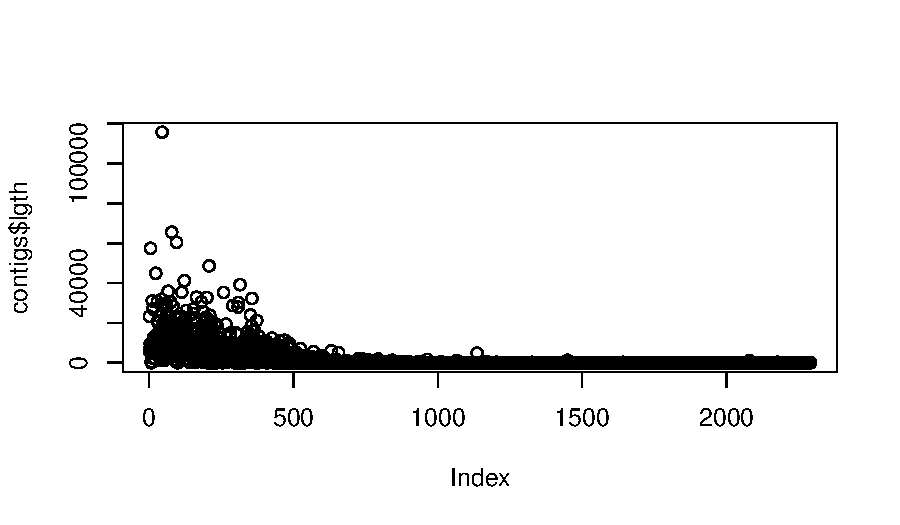
\includegraphics{plots/figura-024}
\end{frame}

\subsection{Lines}

\begin{frame}[fragile, allowframebreaks]
  \frametitle{Lines}
  \scriptsize 
\begin{Schunk}
\begin{Sinput}
> plot(log10(sort(contigs$lgth)), 
+     type = "l")
> lines(log10(1:length(contigs$lgth)^2), 
+     col = "red")
\end{Sinput}
\end{Schunk}
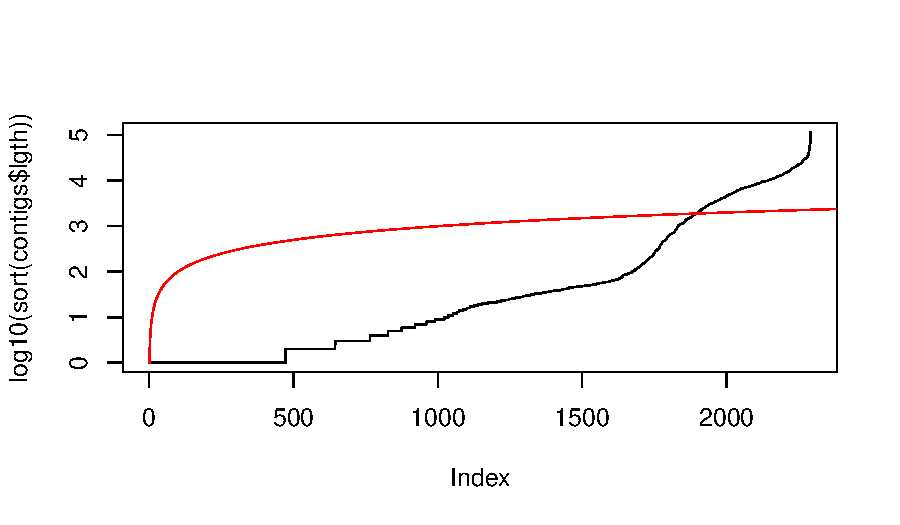
\includegraphics{plots/figura-025}
\normalsize
\end{frame}

\subsection{Barplot}

\begin{frame}[fragile, allowframebreaks]
  \frametitle{Barplot}
  \scriptsize 
\begin{Schunk}
\begin{Sinput}
> barplot(contigs$lgth[contigs$lgth > 
+     30000]/1000, col = rainbow(length(contigs$lgth[contigs$lgth > 
+     30000])), xlab = "Contigs larger than 30kb", 
+     ylab = "Length in kb", main = "Largest contigs")
\end{Sinput}
\end{Schunk}
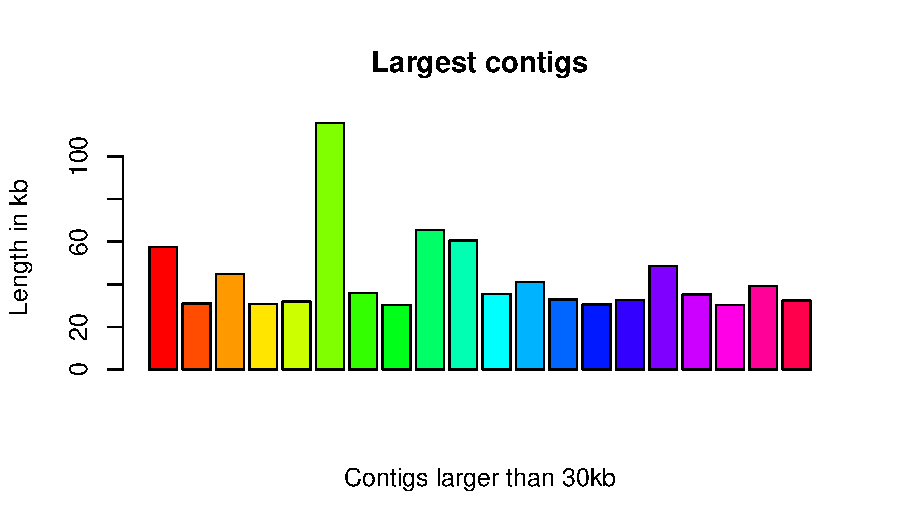
\includegraphics{plots/figura-026}
\normalsize
\end{frame}

\subsection{Histogram}

\begin{frame}[fragile, allowframebreaks]
  \frametitle{Basic histogram}
\begin{Schunk}
\begin{Sinput}
> hist(contigs$lgth, col = "lightblue")
\end{Sinput}
\end{Schunk}
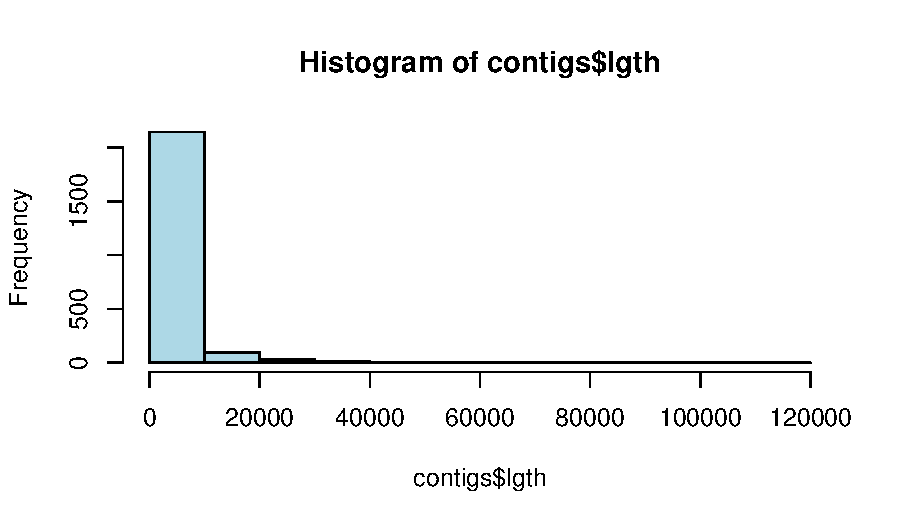
\includegraphics{plots/figura-027}
\end{frame}

\subsection{Density}

\begin{frame}[fragile, allowframebreaks]
  \frametitle{Plotting the density}
\begin{Schunk}
\begin{Sinput}
> hist(contigs$lgth, col = "lightblue", 
+     prob = T)
> lines(density(contigs$lgth), col = "red")
\end{Sinput}
\end{Schunk}
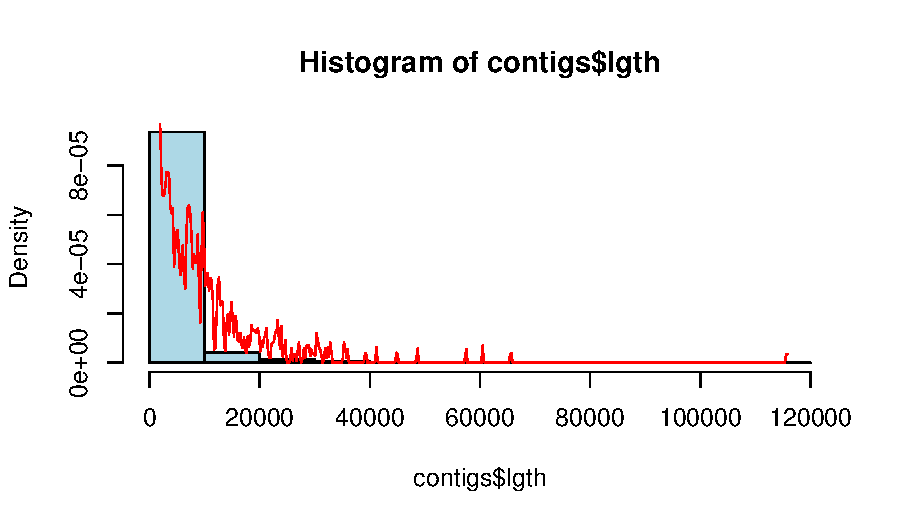
\includegraphics{plots/figura-028}
\end{frame}

\subsection{Boxplot}

\begin{frame}[fragile, allowframebreaks]
  \frametitle{Graphical view of the summary}
\begin{Schunk}
\begin{Sinput}
> boxplot(contigs$lgth, rnorm(1000, 
+     40000, 10000), col = c("lightblue", 
+     "red"))
\end{Sinput}
\end{Schunk}
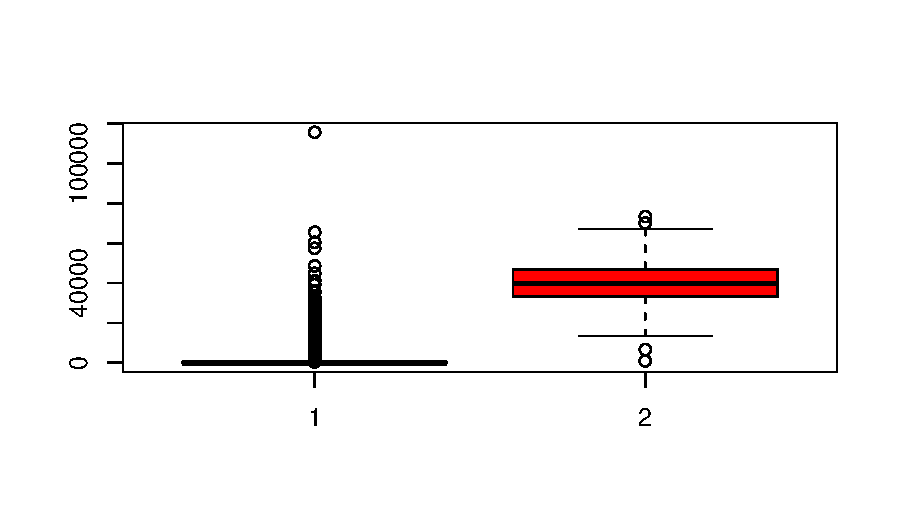
\includegraphics{plots/figura-029}
\end{frame}


\subsection{Mosaicplot}

\begin{frame}[fragile, allowframebreaks]
  \frametitle{Great for table with 3 dims}
\begin{Schunk}
\begin{Sinput}
> mosaicplot(HairEyeColor, shade = TRUE)
\end{Sinput}
\end{Schunk}
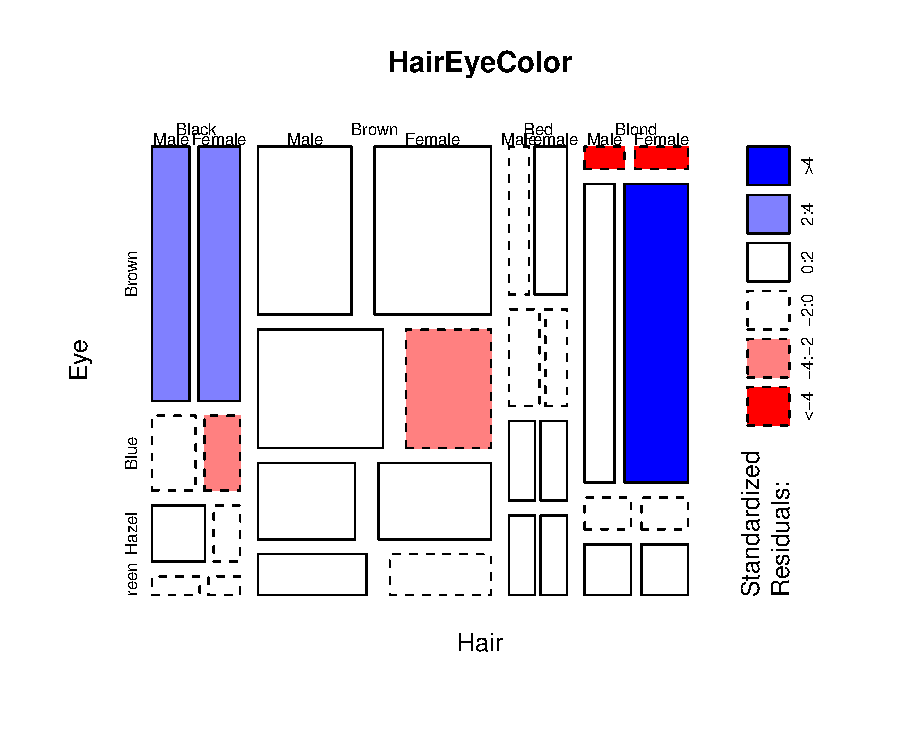
\includegraphics{plots/figura-030}
\end{frame}

\subsection{Image}

\begin{frame}[fragile, allowframebreaks]
  \frametitle{Helps visualize your matrix}
\begin{Schunk}
\begin{Sinput}
> x <- matrix(1:100, 10, 10, byrow = T)
> image(x, col = heat.colors(100))
\end{Sinput}
\end{Schunk}
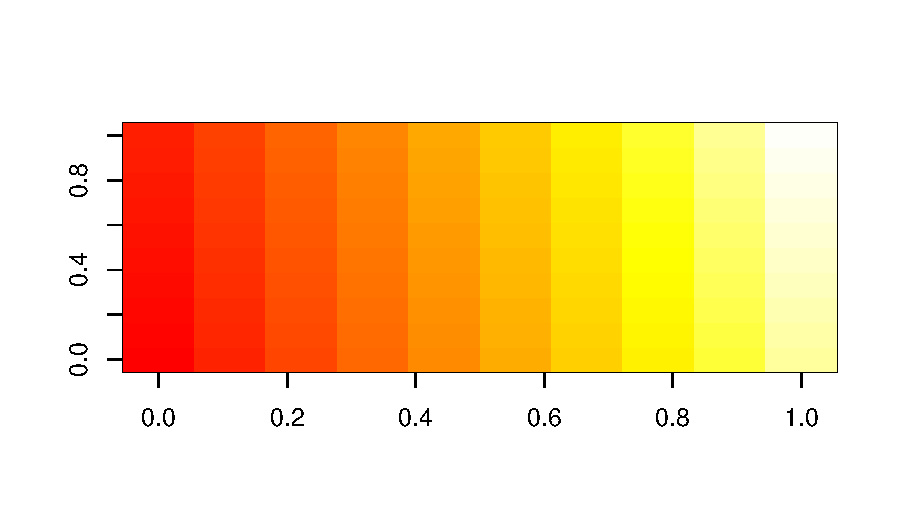
\includegraphics{plots/figura-031}
\end{frame}

\subsection{PDF and PNG}

\begin{frame}[allowframebreaks, fragile]
  \frametitle{Exporting images}
  \begin{itemize}
  \item You can always export your images into PDF or PNG files.
\begin{Schunk}
\begin{Sinput}
> pdf(file = "file.pdf", onefile = T)
> plot("some data")
> dev.off()
> png(file = "image.png")
> plot("some data")
> dev.off()
\end{Sinput}
\end{Schunk}
  \end{itemize}
\end{frame}


%%%%%%%%%%%%%%%%%%%%%%%%%%%%%%%%%%%%%%%%%%%%%%%%%%%%%%%%%%%%%%%%%%%%%%%%%%%
\section{Flow control}

\begin{frame}[allowframebreaks, fragile]
  \frametitle{Two options}
  \begin{itemize}
  \item \BIOCfunction{While} is quite easy to use: \pl{while (cond) expr}
\begin{Schunk}
\begin{Sinput}
> x <- NULL
> while (length(x) < 10) {
+     x <- c(x, runif(1))
+ }
\end{Sinput}
\end{Schunk}
  \item What is the length of the \pl{x} object? Now lets use \BIOCfunction{repeat} with \BIOCfunction{break}.
  \item With \pl{while} and \pl{repeat} be careful to avoid \alert{infinite loops!}
\begin{Schunk}
\begin{Sinput}
> x <- 1
> repeat {
+     x <- x + 2
+     print(x)
+     if (x > 10) 
+         break
+ }
\end{Sinput}
\begin{Soutput}
[1] 3
[1] 5
[1] 7
[1] 9
[1] 11
\end{Soutput}
\end{Schunk}
  \end{itemize}
\end{frame}

\begin{frame}[allowframebreaks, fragile]
  \frametitle{An alternative}
  \begin{itemize}
  \item The most widely used form of iteration is the \alert{for} cycle: \pl{for (var in seq) expr}
\begin{Schunk}
\begin{Sinput}
> for (i in seq_len(3)) print(i)
\end{Sinput}
\begin{Soutput}
[1] 1
[1] 2
[1] 3
\end{Soutput}
\begin{Sinput}
> for (i in letters[4:6]) print(i)
\end{Sinput}
\begin{Soutput}
[1] "d"
[1] "e"
[1] "f"
\end{Soutput}
\end{Schunk}
  \item Using \pl{seq\_len} is recommended versus using \pl{1:length(object)}
  \item As you might want to use conditionals \BIOCfunction{if}, \BIOCfunction{ifelse} and \BIOCfunction{switch} could be of your interest.
  \end{itemize}
\end{frame}

\subsection{Creating functions}

\begin{frame}[allowframebreaks, fragile]
  \frametitle{Basis}
  \begin{itemize}
  \item Its quite easy to write your own \pl{R} functions using \BIOCfunction{function}.
  \item While it can take several arguments as input, it only returns \alert{one} object which can be a vector.
  \item The object returned is either the last one to be evaluated or the one specified with \BIOCfunction{return}. 
  \item Say you use an argument x inside a function, this one will not be related to a variable x outside the function.\footnote{For more curious users, look for guides on environments}
\begin{Schunk}
\begin{Sinput}
> x <- 5
> y <- function(x) rnorm(x)
> y(2)
\end{Sinput}
\begin{Soutput}
[1] -1.1001290 -0.4363984
\end{Soutput}
\begin{Sinput}
> x
\end{Sinput}
\begin{Soutput}
[1] 5
\end{Soutput}
\end{Schunk}
  \end{itemize}
\end{frame}

\subsection{Apply functions}

\begin{frame}[allowframebreaks, fragile]
  \frametitle{A neat family}
  \begin{itemize}
  \item Their main utility is to \emph{apply} a function to all the elements of an object. Say all the columns of a matrix.
  \item In most cases, the return value is simplified and in others its an argument.
  \item Its easier for someone to understand a code with \BIOCfunction{apply} functions than \pl{for} loops.
\begin{Schunk}
\begin{Sinput}
> mat <- matrix(rnorm(100), 10, 10)
> apply(mat, 1, sum)
\end{Sinput}
\begin{Soutput}
 [1] -3.3583902  0.8250018  3.9749494
 [4]  0.8761072 -2.6867082 -0.5183255
 [7] -1.2522203  0.4885079 -0.5388356
[10] -0.2917741
\end{Soutput}
\end{Schunk}
  \item Keep in mind that some \pl{R} functions are way faster than using apply, such as \BIOCfunction{rowMeans}.
\begin{Schunk}
\begin{Sinput}
> apply(mat, 1, sum) == rowSums(mat)
\end{Sinput}
\begin{Soutput}
 [1] TRUE TRUE TRUE TRUE TRUE TRUE TRUE
 [8] TRUE TRUE TRUE
\end{Soutput}
\end{Schunk}
  \item Some packages implement new \pl{apply} functions, but here are the common ones:
  \begin{itemize}
  \item \pl{apply} Useful for matrices and data.frames
  \item \pl{lapply} Its the list version
  \item \pl{sapply} Simplest one to use (lists and vectors)
\begin{Schunk}
\begin{Sinput}
> x <- list(rnorm(100), runif(100), 
+     rlnorm(100))
> sapply(x, quantile)
\end{Sinput}
\begin{Soutput}
           [,1]       [,2]       [,3]
0%   -2.7540348 0.03099712  0.1231390
25%  -0.7164680 0.31074536  0.5880255
50%   0.1520818 0.54236418  0.9720055
75%   0.8725263 0.71203283  2.2368822
100%  2.3792556 0.99192278 11.6742964
\end{Soutput}
\end{Schunk}
  \item \pl{tapply} Uses a vector and a factor, great for grouped data
\begin{Schunk}
\begin{Sinput}
> x <- data.frame(info = rnorm(10), 
+     group = as.factor(sample(1:3, 
+         10, replace = T)))
> tapply(x$info, x$group, mean)
\end{Sinput}
\begin{Soutput}
         1          2          3 
-0.2252659  0.7718850 -0.6408342 
\end{Soutput}
\end{Schunk}
  \item \pl{eapply} For environments and the curious ones
  \item \pl{mapply} Multivariate version of \pl{sapply}
\begin{Schunk}
\begin{Sinput}
> mapply(rep, 1:4, 4:1)
\end{Sinput}
\begin{Soutput}
[[1]]
[1] 1 1 1 1

[[2]]
[1] 2 2 2

[[3]]
[1] 3 3

[[4]]
[1] 4
\end{Soutput}
\end{Schunk}
  \item \pl{rapply} Recursive version of \pl{lapply}
  \end{itemize}
  \item You might find this site useful: \myurlshort{www.ats.ucla.edu/stat/r/library/advanced\_function\_r.htm}{advanced\_function\_r.htm}
  \end{itemize}
\end{frame}

%%%%%%%%%%%%%%%%%%%%%%%%%%%%%%%%%%%%%%%%%%%%%%%%%%%%%%%%%%%%%%%%%%%%%%%%%%%
\section{Exercises}

\begin{frame}[allowframebreaks]
  \frametitle{or homework :P}
  \begin{itemize}
  \item Please go to the \myurlshort{www.lcg.unam.mx/~lcollado/B/}{official course site} and complete the first exercise file.
  \item Homework specifications are available on the \pl{Course Syllabus}. 
  \begin{itemize}
    \item For this homework only hand in a portable \pl{.R} file with comments. Next week we'll learn about \pl{Sweave} and \emph{vignette} files.
  \end{itemize}
  \end{itemize}
\end{frame}


\end{document}
